\documentclass[12pt]{article}

\usepackage{booktabs}% http://ctan.org/pkg/booktabs
\usepackage[utf8]{inputenc}
\usepackage{changepage}
\usepackage{pgfplots}
\usepackage{amssymb}
\usepackage{xcolor}
\usepackage{hyperref}
\usepackage{listings}
\usepackage[T1]{fontenc}
\usepackage[utf8]{inputenc}
\usepackage{adjustbox}
\usepackage{amsmath}
\usepackage{mathtools}
\usepackage{biblatex}
\lstset{
  language=Python,
  numbers=left,
  numberstyle=\tiny,
  stepnumber=1,
  numbersep=5pt,
  tabsize=4,
  basicstyle=\ttfamily,
  columns=fullflexible,
  keepspaces,
}
\hypersetup{
    colorlinks,
    citecolor=black,
    filecolor=black,
    linkcolor=black,
    urlcolor=black
}

% Set page size and margins
% Replace `letterpaper' with `a4paper' for UK/EU standard size
\usepackage[letterpaper,top=2cm,bottom=2cm,left=3cm,right=3cm,marginparwidth=1.75cm]{geometry}

% Useful packages
\usepackage{amsmath}
\usepackage{mathtools}
\usepackage{graphicx}
\newenvironment{para}{\begin{adjustwidth}{13mm}{}}{\end{adjustwidth}}

\newcommand\tab[1][1cm]{\hspace*{#1}}

\newcommand{\tabitem}{\llap{\textbullet}}
\newcommand{\Hsquare}{%
\text{\fboxsep=-.2pt\fbox{\rule{0pt}{1ex}\rule{1ex}{0pt}}}%
}

\newtheorem{Definizione}{Definizione}[subsection]
\newtheorem{Lemma}{Lemma}[subsection]
\newtheorem{Teorema/Definizione}{Teorema/Definizione}[subsection]
\newtheorem{Corollario}{Corollario}[subsection]
\newtheorem{Teorema}{Teorema}[subsection]
\newtheorem{Proposizione}{Proposizione}[subsection]
\newtheorem{Notazione}{Notazione}[subsection]
\newtheorem{Commento}{Commento}[subsection]
\newtheorem{Dimostrazione}{Dimostrazione}[subsection]
\newtheorem{Osservazione}{Osservazione}[subsection]
\newtheorem{Nota}{Nota}[subsection]


\title{Analisi e Progettazione del Software}
\author{spitfire}
\date{A.A. 2023-2024}
\begin{document}
\begin{figure}
    \centering
    
\includegraphics[width=0.35\textwidth]{Images/Logo scienze bicocca.png}
\end{figure}

\vspace{10cm}
\date{A.A. 2023-2024}


\maketitle

\newpage

\tableofcontents
\newpage

\section{Introduzione}
Che cos'è il \textbf{software}? Esso è \textbf{un programma per computer} unito alla \textbf{documentazione ad esso associata},
la quale specifica e comprende \textbf{requisiti, modelli di progetto, manuale utente,...} \newline
I prodotti software possono essere:
\begin{itemize}
    \item \textbf{Generici}: sviluppati per un ampio insieme di clienti (elaboratori di testo, database,...)
    \item \textbf{Personalizzati} (custom): sviluppati per un singolo cliente in base alla sue esigenze specifiche
\end{itemize}
Un nuovo prodotto software può essere \textbf{creato da zero, personalizzando software già esistenti o riusando parti o software già esistente}.
Le caratteristiche essenziali di un buon software sono:
\begin{center}
    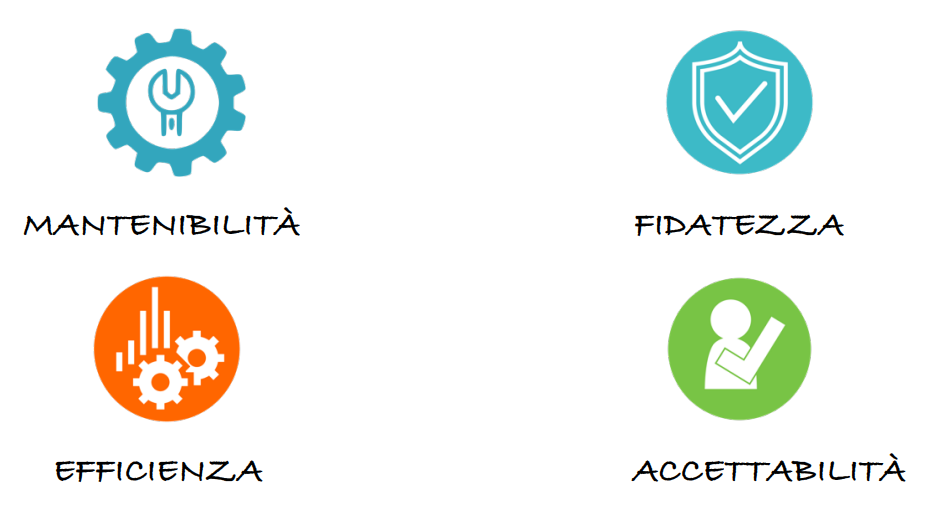
\includegraphics[width = 0.80\textwidth]{Images/1.png}
\end{center}
\subsection{Introduzione all'ingegneria del software}
Che cos'è \textbf{l'ingegneria del software}? \textbf{L'ingegneria del software} è una disciplina ingegneristica che si occupa
di tutti gli aspetti della produzione del software di buona qualità, dalle \textbf{prime fasi della specifica del sistema fino alla manutenzione del sistema}
dopo la messa in uso. Vediamo cosa si intende per \textbf{disciplina ingegneristica} e "\textbf{Tutti gli aspetti della produzione del software}":
\begin{itemize}
    \item \textbf{Disciplina ingegneristica}: Utilizzare metodi e teorie \textbf{appropriati} per risolvere i problemi tenendo conto dei vincoli \textbf{organizzativi e finanziari}
    \item \textbf{Tutti gli aspetti della produzione del software}: Non solo il \textbf{processo tecnico di sviluppo}. Anche la \textbf{gestione del progetto} e lo sviluppo di \textbf{strumenti}
    ,metodi ecc... per supportare la produzione del software
\end{itemize}
\newpage
\noindent
La disciplina dell'ingegneria del software si occupa di:
\begin{center}
    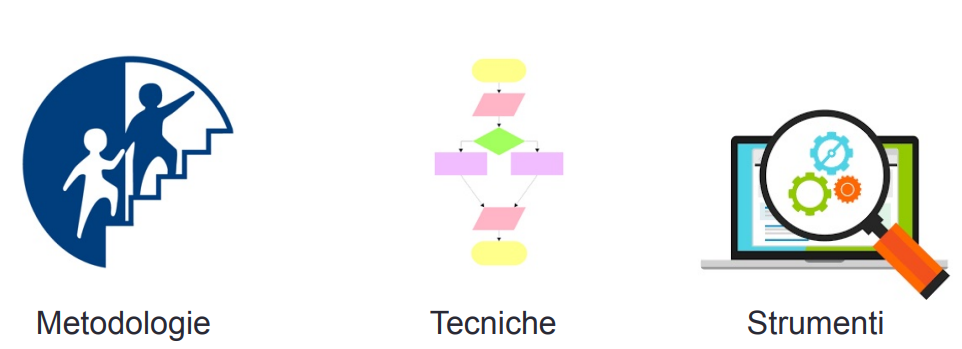
\includegraphics[width = 0.80\textwidth]{Images/2.png}
\end{center}
\subsection{La crisi del software}
Il termine \textbf{crisi del software} (o software crisis) è usato nell'ambito dell'ingegneria del software per descrivere l'impatto della \textbf{rapida crescita} della potenza degli elaboratori
e la \textbf{complessità} dei problemi che dovevano esseri affrontati. Le parole chiavi della software crisis erano \textbf{complessità, attese e cambiamento}. Il concetto di software crisis emerse negli
anni '60.
\begin{center}
    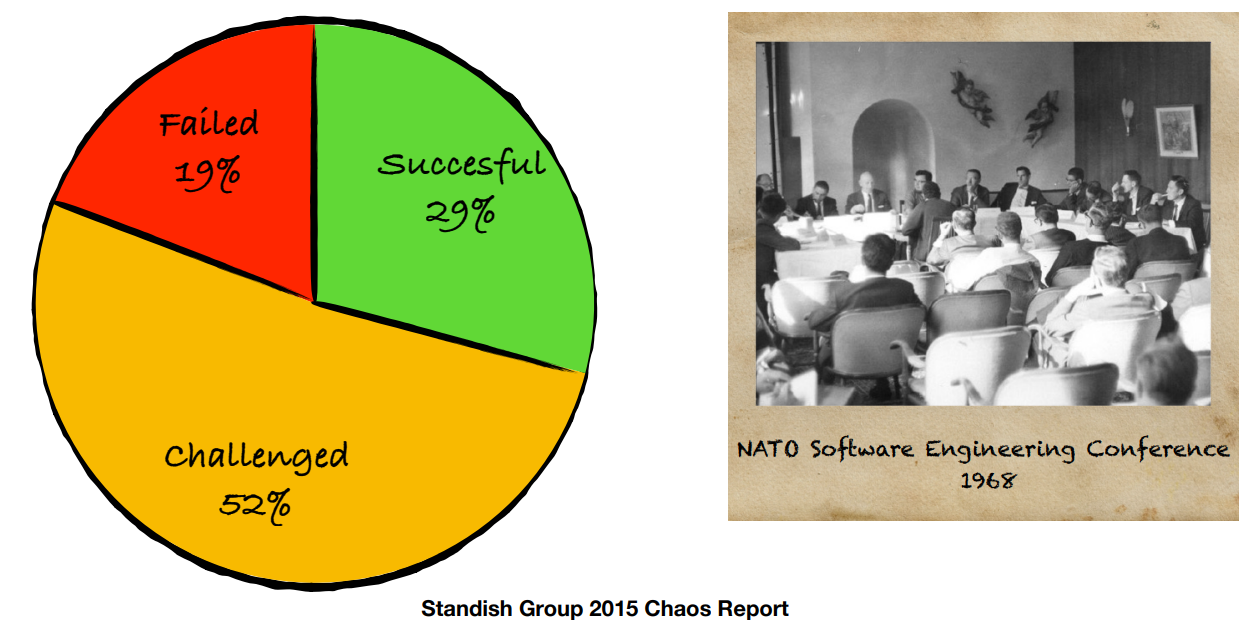
\includegraphics[width = 0.80\textwidth]{Images/3.png}
\end{center}
\begin{center}
    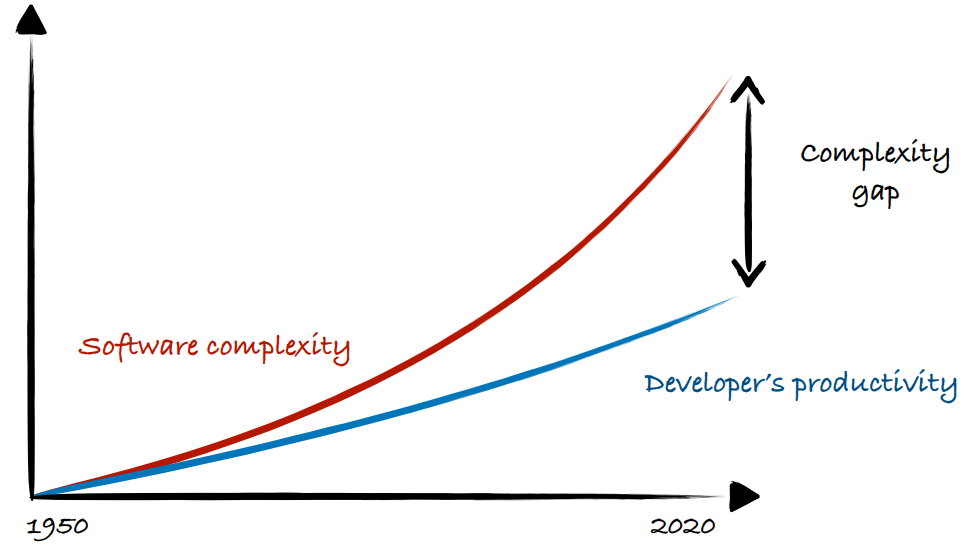
\includegraphics[width = 0.80\textwidth]{Images/4.png}
\end{center}
Le cause della crisi del software erano legate alla \textbf{complessità dei processi software} e alla \textbf{relativa immaturità dell'ingegneria del software}
Per superare la crisi infatti si dovettero introdurre:
\begin{itemize}
    \item \textbf{Management}
    \item \textbf{Organizzazione}, attraverso \textbf{analisi e progettazione}
    \item \textbf{Teorie e tecniche} come la \textbf{programmazione strutturata e ad oggetti}
    \item \textbf{Strumenti}, come gli IDE
    \item \textbf{Metodologie}, tra cui il \textbf{modello a cascata e il modello agile}
\end{itemize}
\subsection{Analisi e progettazione}
Che cosa sono \textbf{analisi e progettazione}? \newline
\textbf{L'analisi} enfatizza un'\textbf{investigazione del problema e dei requisiti} invece che una soluzione: per esempio, se si vuole realizzare un nuovo sistema di trading online,
bisognerà capire \textbf{come questo sistema verrà utilizzato} e \textbf{quali sono le sue funzioni}. "Analisi" è un termine ampio con più accezioni, tra cui:
\begin{itemize}
    \item \textbf{Analisi dei requisiti}, cioè un'investigazione dei requisiti del sistema
    \item \textbf{Analisi orientata agli oggetti}, cioè un'investigazione degli oggetti di dominio
\end{itemize} 
La \textbf{progettazione} enfatizza una soluzione \textbf{concettuale} (software e hardware) che \textbf{soddisfa i requisiti}, anziché la relativa implementazione. Per esempio, la descrizione di uno schema di base di dati
e di oggetti software. Nella progettazione vengono spesso \textbf{esclusi dettagli di basso livello o "ovvi"} (o almeno "ovvi" per coloro a cui è destinato il software). \newline
Infine i progetti possono essere \textbf{implementati} e la loro implementazione (ovvero il codice) esprime il progetto realizzato vero e completo.
Come nel caso dell'analisi, anche "progettazione" è un termine con più accezioni, tra cui:
\begin{itemize}
    \item \textbf{Progettazione orientata agli oggetti}
    \item \textbf{Progettazione di basi di dati}
\end{itemize}
L'analisi e la progettazione possono essere riassunti con la seguente frase:
\begin{center}
    \textbf{Fare la cosa giusta}(analisi) \textbf{e fare la cosa bene}(progettazione)
\end{center}
\subsubsection{Analisi e progettazione orientata agli oggetti}
Durante \textbf{l'analisi orientata agli oggetti} c'è un enfasi sull'\textbf{identificazione} e la \textbf{descrizione degli oggetti}, o dei \textbf{concetti}, nel \textbf{dominio del problema}.
Per esempio, nel caso di un sistema informatico per voli aerei, alcuni dei concetti possono essere \textit{Aereo, Volo} e \textit{Pilota}. \newline
Durante \textbf{la progettazione orientata agli oggetti} (o più semplicemente \textbf{progettazione a oggetti}) l'enfasi è sulla \textbf{definizione di oggetti software} e sul \textbf{modo in cui questi collaborano
per soddisfare i requisiti}. Per esempio un oggetto software \textit{Aereo} può avere un attributo \textit{codiceDiRegistrazione} e un metodo \textit{getVoliEffettuati}. \newline
\begin{center}
    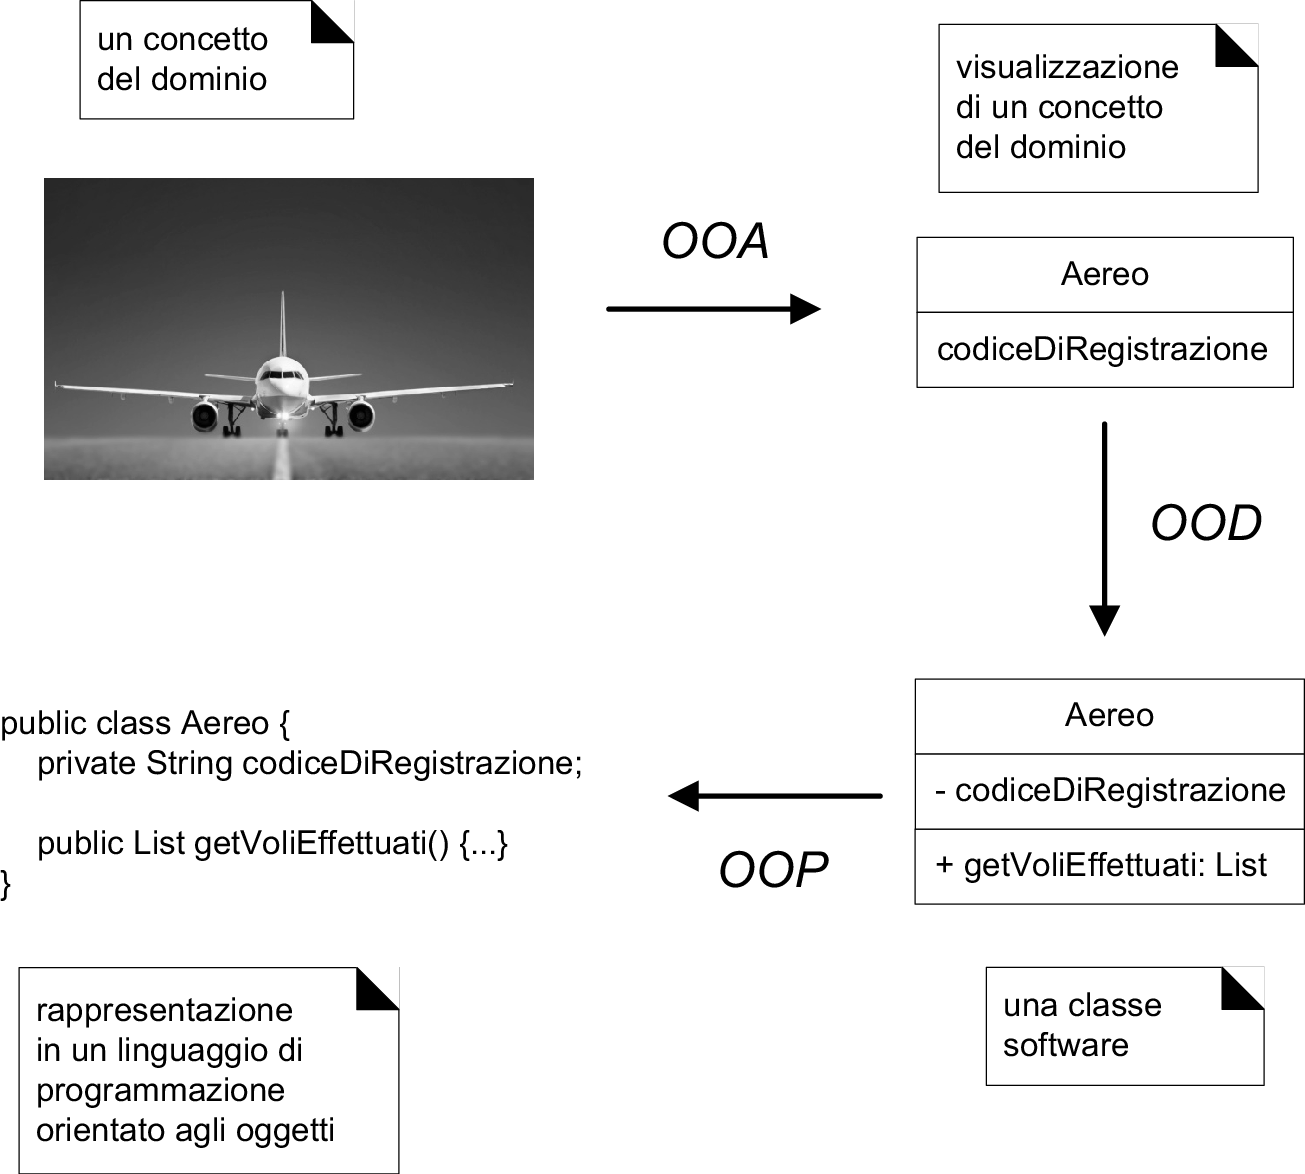
\includegraphics[width = 0.70\textwidth]{Images/5.png}
\end{center}
Infine durante \textbf{l'implementazione} o la \textbf{programmazione orientata agli oggetti}, gli oggetti progettati vengono implementati, per esempio implementando la classe \textit{Aereo} in un linguaggio ad oggetti.
Dunque, analisi e progettazione \textbf{hanno obbiettivi diversi che vengono perseguiti in maniera diversa}. Tuttavia, come mostrato dall'esempio sopra, esse sono \textbf{attività fortemente sinergiche} che sono \textbf{correlate fra loro}
e con le \textbf{altre attività dello sviluppo del software}.
\subsection{Introduzione ai diagrammi e ai passi fondamentali dello sviluppo software}
Vediamo una breve introduzione dei \textbf{vai diagrammi e dei passi fondamentali} legati allo sviluppo software.
\begin{center}
    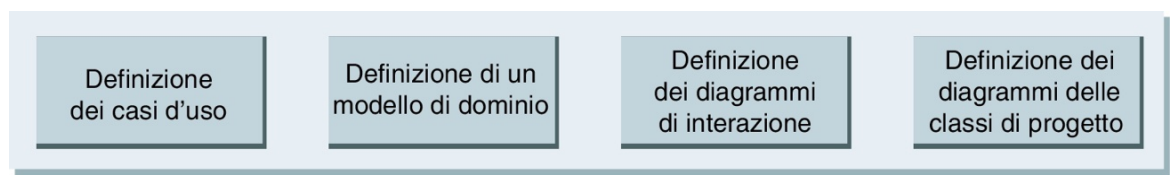
\includegraphics[width = 0.80\textwidth]{Images/6.png}
\end{center}
\subsubsection{Definizione dei casi d'uso}

\textbf{L'analisi dei requisiti} può comprendere \textbf{storie o scenari} relativi al modo in cui l'applicazione può essere utilizzata dagli utenti;
queste storie possono essere scritte come \textbf{casi d'uso}. I casi d'uso \textbf{non sono un elaborato ad oggetti} ma semplicemente delle storie scritte. Sono tuttavia
uno strumento \textbf{diffuso nell'analisi dei requisiti}. Facciamo un'esempio: \newline
\textbf{Gioca una partita a Dadi}: Il giocatore chiede di lanciare i dadi. Il Sistema presenta il risultato: se il valore totale delle facce dei dadi è sette, il giocatore ha vinto; altrimenti ha perso.
\subsubsection{Definizione di un modello di dominio}
L'analisi orientata agli oggetti è interessata alla \textbf{creazione di una descrizione del dominio da un punto di vista ad oggetti}. Vengono identificati i \textbf{concetti, gli attributi e le associazioni considerati significativi}.
Il risultato può essere espresso come un \textbf{modello di dominio} che mostra i concetti o gli oggetti \textbf{significativi} del dominio. Esso è rappresentato nel seguente modo:
\begin{center}
    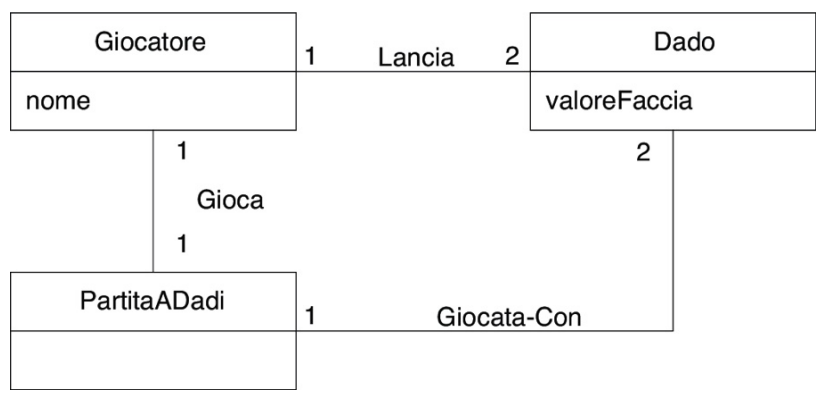
\includegraphics[width = 0.65\textwidth]{Images/7.png}
\end{center}
\subsubsection{Definizione dei diagrammi di interazione}
La \textbf{progettazione ad oggetti} è interessata alla \textbf{definizione di oggetti software, delle loro responsabilità e collaborazioni}. Una notazione comune per illustrare queste collaborazione è un
\textbf{diagramma di sequenza} (un tipo di diagramma UML). Esso mostra lo scambio di messaggi \textbf{tra oggetti software}, dunque l'invocazione di \textbf{metodi}. Esso è rappresentato nel seguente modo:
\begin{center}
    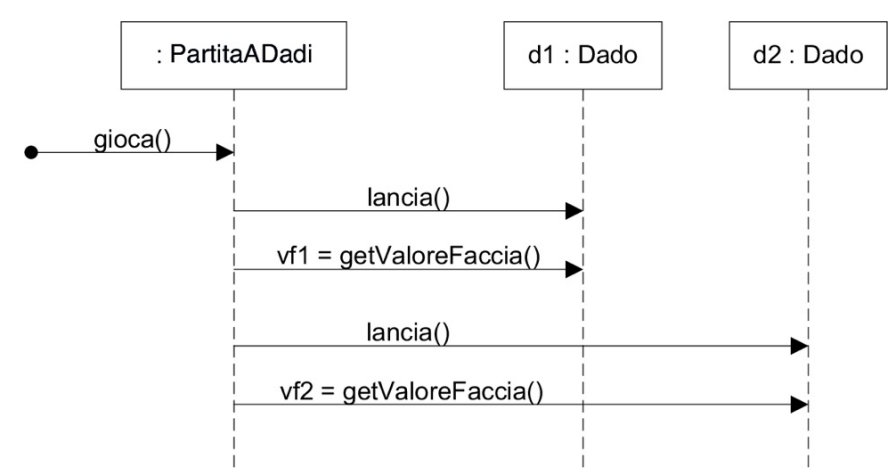
\includegraphics[width = 0.65\textwidth]{Images/8.png}
\end{center}
È interessante notare come \textbf{la progettazione degli oggetti software e dei programmi si può ispirare a un dominio del mondo reale}, tuttavia essa non è \textbf{nè un modello diretto nè una simulazione di questo dominio}. Quindi, per esempio,
seppur nel mondo reale è il giocatore a lanciare il dado, nel progetto software è l'oggetto \textit{PartitaADadi} che "lancia" i dadi.
\subsubsection{Definizione dei diagrammi di classe di progetto}
Accanto a una visione dinamica delle \textbf{collaborazioni tra oggetti}, mostrata dai diagrammi di interazione, è utile mostrare una \textbf{vista statica} delle definizioni di classi mediante un \textbf{diagramma delle classi di progetto}, che mostra le classi software 
con i loro attributi e metodi. Il diagramma delle classi di progetto è rappresentato nella seguente maniera:
\begin{center}
    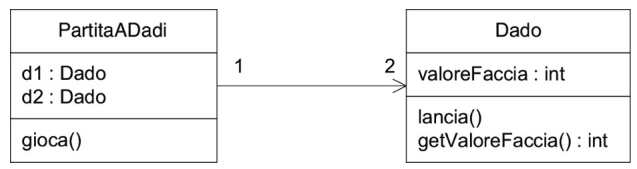
\includegraphics[width = 0.65\textwidth]{Images/9.png}
\end{center}
Diversamente dal modello di dominio, che illustra \textbf{classi del mondo reale}, questo diagramma mostra \textbf{classi software}.
Si noti che, benché questo diagramma delle classi di progetto \textbf{non sia uguale al modello di dominio}, i nomi e il contenuto delle classi sono \textbf{simili}. In tal modo i \textbf{progetti e i linguaggi Object Oriented} (OO) sono in grado di \textbf{favorire un salto rappresentazionale basso}
tra i componenti software e il nostro modello mentale di un dominio, \textbf{migliorando la comprensione}.
\subsection{UML}
\textbf{Unified Modelling Language}, abbreviato \textbf{UML}, è un \textbf{linguaggio visuale} per la \textbf{specifica, la costruzione e la documentazione degli elaborati} di un sistema software.
UML rappresenta una \textbf{collezione di best practices di ingegneria}, dimostratesi vincenti nella modellazione di sistemi vasti e complessi; inoltre esso \textbf{favorisce la divulgazione delle informazioni nella comunità dell'ingegneria del software} in quanto è \textit{standard de facto}.
Bisogna però tenere a mente che \textbf{UML non è una metodologia ma un linguaggio!} \newline
Il termine \textit{visuale} della definizione è un punto fondamentale. UML è uno standard de facto per la \textbf{notazione di diagrammi per disegnare o rappresentare figure} (con del testo) \textbf{relative al software}, e in particolare, al software OO.
A un livello più profondo, di particolare interesse per i produttori di strumenti per \textbf{MDA} (Model Driven Architecture) alla base della notazione UML c'è il \textbf{meta-modello di UML} che descrive la \textbf{semantica} degli elementi di modellazione, tuttavia non è necessario che lo sviluppatore lo conosca. 
Presentiamo ora una breve storia di UML:
\begin{center}
    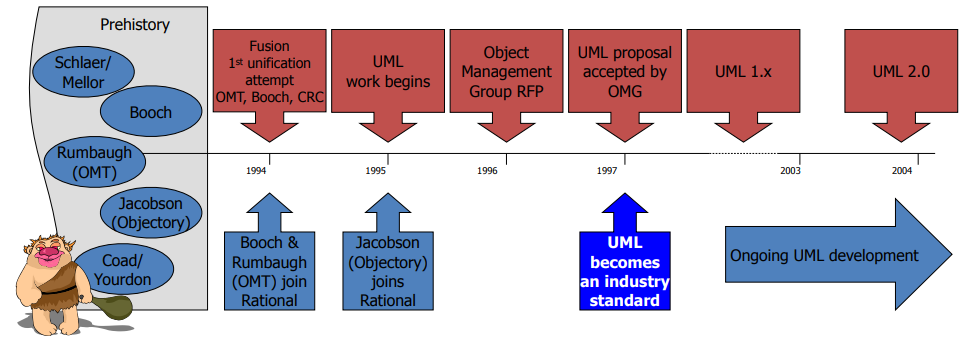
\includegraphics[width = 1.05\textwidth]{Images/10.PNG}
\end{center}
Il più significativo aggiornamento di UML è avvenuto nel \textbf{2003}:
\begin{itemize}
    \item Maggiore \textbf{consistenza}
    \item Semantica definita in maniera \textbf{più chiara e dettagliata}
    \item \textbf{Nuovi diagrammi}
    \item Compatibilità con le precedenti versioni (1.x)
\end{itemize}
Altra parola importante è \textit{unified}: UML vuole essere un \textbf{linguaggio unificante} sotto diversi aspetti:
\begin{itemize}
    \item \textbf{Storico} (OMT, Booch, CRC, Objectory)
    \item \textbf{Ciclo di sviluppo} (sintassi visuali per tutte le fasi)
    \item \textbf{Domini applicativi} (dai sistemi embedded ai sistemi gestionali)
    \item \textbf{Linguaggi e piattaforme di sviluppo} (.Net, Java, C\#,...)
    \item \textbf{Processi di sviluppo} (UP, BPM, ...)
\end{itemize}
\subsubsection{UML e gli oggetti}
UML modella i sistemi come \textbf{una serie di oggetti che collaborano fra loro}. Si hanno quindi due strutture:
\begin{itemize}
    \item \textbf{Struttura statica}:
    \begin{itemize}
        \item \textbf{Quali} tipi di oggetti sono necessari
        \item \textbf{Come} sono correlati
    \end{itemize}
    \item \textbf{Struttura dinamica}:
    \begin{itemize}
        \item \textbf{Ciclo di vita} di questi oggetti
        \item \textbf{Come collaborano} per fornire le funzionalità richieste
    \end{itemize}
\end{itemize}
\subsubsection{Tre modi di applicare UML}
\textbf{Fowler} [Fowler03] descrive tre modi per applicare UML:
\begin{itemize}
    \item \textbf{UML come abbozzo}: Diagrammi \textbf{informali e incompleti} (spesso abbozzati a mano su una lavagna bianca), che vengono creati per 
    \textbf{esplorare parti difficili dello spazio del problema o della soluzione}, sfruttando l'espressività dei linguaggi visuali.
    \item \textbf{UML come progetto}: Diagrammi di progetto abbastanza dettagliati che vengono utilizzati per:
    \begin{enumerate}
        \item \textbf{Il reverse engineering}, ovvero per visualizzare e comprendere meglio \textbf{del codice già esistente} mediante dei diagrammi UML. In questo caso, uno strumento UML legge il codice
        sorgente o binario per \textbf{generare} (di solito) \textbf{dei diagrammi UML dei package, delle classi e di sequenza}. Questi "progetti" possono aiutare il lettore a capire i principali elementi, le strutture e le collaborazioni
        \item \textbf{Il forward engineering}, ovvero per la \textbf{generazione di codice}. In questo caso, alcuni diagrammi dettagliati possono fornire una \textbf{guida alla generazione di codice} da fare manualmente o automaticamente con un strumento.
        Solitamente, i diagrammi sono utilizzati per \textbf{specificare una parte di codice}, mentre il resto del codice viene scritto da uno sviluppatore durante la codifica, magari applicando UML come abbozzo.
    \end{enumerate}
    \item \textbf{UML come linguaggio di programmazione}: La specifica \textbf{completamente eseguibile} di un sistema software con UML.
    Il codice viene generato \textbf{automaticamente} e non viene normalmente normalmente né visto né modificato dagli sviluppatori; quindi UML viene usato come vero e proprio \textbf{linguaggio di programmazione}.
    Questo utilizzo di UML richiede un modo \textbf{pratico} per rappresentare sotto forma di di diagrammi \textbf{tutto il comportamento o la logica} (probabilmente tramite diagrammi di interazione e di stato).
    Si tratta di un approccio \textbf{ancora in corso di sviluppo} sia in termini di teoria sia in termini di usabilità e robustezza degli strumenti.
\end{itemize}
La \textbf{modellazione agile} enfatizza l'uso di UML come \textbf{abbozzo}; si tratta di un metodo comune per applicare UML, spesso con un elevato ritorno in termini di \textbf{investimento di tempo} (che è normalmente breve).
\subsubsection{Due punti di vista per applicare UML}
UML descrive dei tipi \textbf{grezzi} di diagrammi, come i diagrammi delle classi e i diagrammi di sequenza; tuttavia UML \textbf{non impone un particolare punto di vista di modellazione per l'uso di questi diagrammi}; 
quindi la stessa notazione può essere usata secondo \textbf{due punti di vista} (o prospettive) e \textbf{tipi di modelli}:
\begin{itemize}
    \item \textbf{Punto di vista concettuale}: I diagrammi sono scritti e interpretati \textbf{come descrizioni di oggetti del mondo reale} o nel dominio di interesse
    \item \textbf{Punto di vista software}: I diagrammi, che utilizzano \textbf{la stessa notazione del punto di vista concettuale}, descrivono astrazioni o componenti software. In particolare, i diagrammi possono descrivere:
    \begin{enumerate}
        \item \textbf{Implementazioni software} con riferimento a una particolare tecnologia
        \item \textbf{Specifiche e interfacce} di componenti software, ma \textbf{indipendentemente} da ogni possible implementazione
    \end{enumerate}
\end{itemize}
\begin{center}
    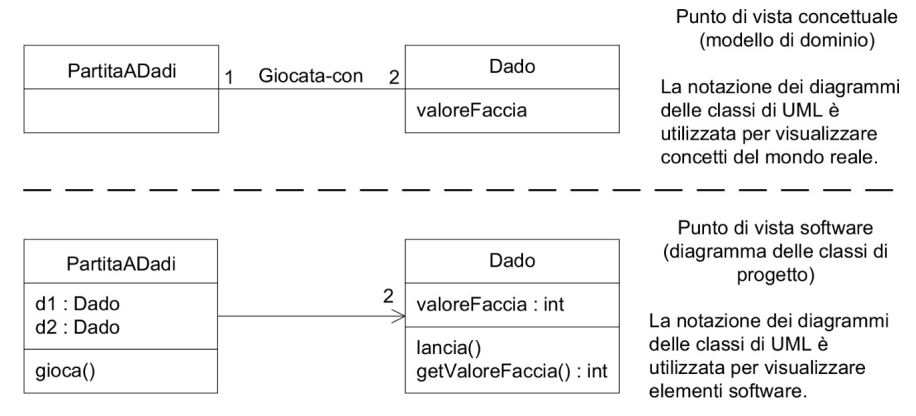
\includegraphics[width = 0.80\textwidth]{Images/11.PNG}
\end{center}
Quindi, in pratica, UMl viene usato:
\begin{enumerate}
    \item \textbf{Nell'analisi}, principalmente secondo il \textbf{punto di vista concettuale}
    \item \textbf{Nella progettazione}, principalmente secondo il \textbf{punto di vista software}
\end{enumerate}
\subsubsection{Significato di classe}
Nell'UML grezzo, abbiamo chiamato "classi" un insieme di oggetti; ma questo termine racchiude una \textbf{varietà di casi}: oggetti fisici, concetti astratti, elementi software, eventi e così via.
In particolare, una classe UML è un caso particolare di un modello UML generale chiamato \textbf{classificatore}, che è qualcosa che ha delle caratteristiche strutturali e/o comportamentali e comprende \textbf{classi, attori, interfacce e casi d'uso}.
Un metodo \textbf{impone una terminologia alternativa sovrapposta all'UML grezzo}; in particolare, ci adegueremo a quella di \textbf{UP} (Unified Process), che chiama:
\begin{itemize}
    \item \textbf{Classe concettuale}: Oggetto o concetto \textbf{del mondo reale} da un punto di vista \textbf{concettuale}. Il modello di dominio di UP contiene \textbf{classi concettuali}
    \item \textbf{Classi software}: Una classe che rappresenta un \textbf{componente software}, da un punto di vista \textbf{software}, indipendentemente dal processo, metodo o linguaggio di programmazione. Il modello di progetto di UP contiene \textbf{classi software}.
\end{itemize}
\subsubsection{Vantaggi della modellazione visuale}
Disegnare e leggere UML implica che si sta lavorando in \textbf{modo visuale}. La modellazione visuale ci permette di sfruttare le capacità del nostro cervello di \textbf{comprendere rapidamente simboli, unità e relazioni nelle notazioni} (prevalentemente bidimensionali) a "rettangoli e linee".
I diagrammi ci aiutano a vedere o esaminare meglio il \textbf{quadro generale} e le relazione tra elementi dell'analisi del software e allo stesso tempo ci permettono di \textbf{ignorare o nascondere i dettagli poco interessanti}.
\section{Processi per lo sviluppo del software}
Un \textbf{processo per lo sviluppo del software} (o \textbf{processo software}) definisce un approccio disciplinato per la \textbf{costruzione}, il \textbf{rilascio} e la \textbf{manutenzione del software}.
Definisce quindi \textbf{chi fa che cosa, quando e come} per raggiungere un certo obbiettivo. In particolare:
\begin{itemize}
    \item \textbf{Cosa} sono le \textbf{attività}
    \item \textbf{Chi} sono i \textbf{ruoli}
    \item \textbf{Come} sono le \textbf{metodologie}
    \item \textbf{Quando} riguarda \textbf{l'organizzazione temporale} delle attività
\end{itemize} 
\newpage
\noindent
Le attività fondamentali di un processo di sviluppo sono:
\begin{center}
    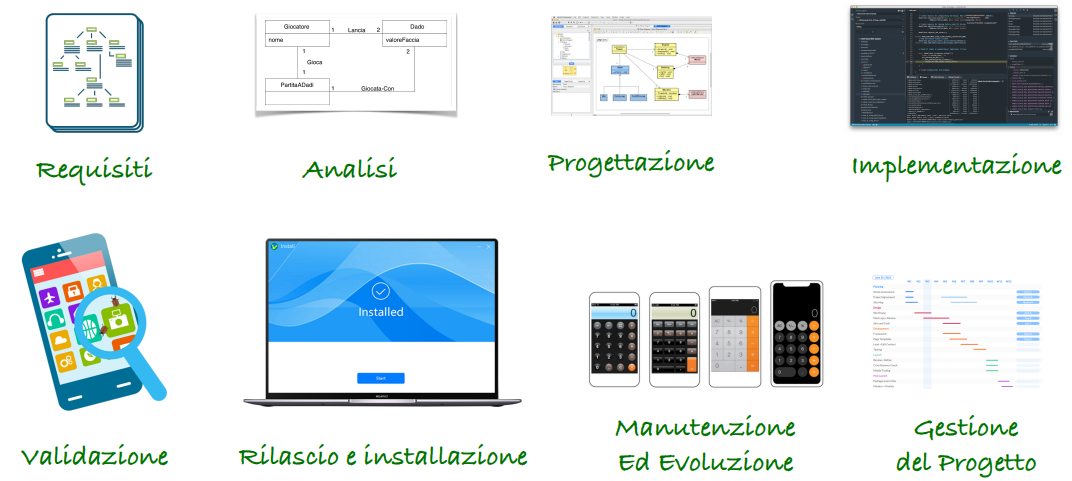
\includegraphics[width = 1\textwidth]{Images/12.PNG}
\end{center}
Ciò che distingue i processi software gli uni dagli altri è tuttavia \textbf{sono le scelte che riguardano l'organizzazione temporale delle attività} (quando), ovvero il modo in cui essi rispondono alle domande:
\begin{itemize}
    \item Per quanto tempo continueremo a svolgere questa attività
    \item Cosa faremo dopo?
\end{itemize}
\subsection{Processi agili e basati sul piano}
I processi \textbf{orientati al piano} sono processi in cui tutte le attività sono \textbf{pianificate in anticipo} e i progressi del progetto sono \textbf{misurati rispetto a questo piano}.
Invece, nei \textbf{processi agili}, la pianificazione è \textbf{incrementale}, quindi risulta più facile modificare il processo per riflettere le mutevoli esigenze del cliente.
In pratica, \textbf{la maggior parte dei processi software include elementi di entrambi gli approcci}. È necessario notare che \textbf{non esistono processi software totalmente sbagliati o corretti}.
\subsection{Modelli di processo software}
In pratica, la maggior parte dei sistemi di grandi dimensioni vengono sviluppati usando processi che incorporano elementi dei seguenti modelli:
\begin{itemize}
    \item \textbf{Sviluppo a cascata}: Modello \textbf{basato sul piano}. Fasi separate di \textbf{specifica} e di \textbf{sviluppo}
    \item \textbf{Sviluppo incrementale}: \textbf{Specifica, sviluppo e validazione} si alternano. Può essere guidato dal piano o agile
    \item \textbf{Integrazione e configurazione}: Il sistema viene assemblato a partire da \textbf{componenti esistenti e configurabili}. Può essere basato sul piano o agile
\end{itemize} 
Tuttavia "\textbf{quale scegliere?}" è una domanda assolutamente non banale. Diamo quindi dei motivi per il quale esistono diversi processi software:
\begin{itemize}
    \item \textbf{Complessità del progetto}: I progetti software possono variare \textbf{in termini di complessità}, da semplici applicazioni a sistemi complessi e "mission-critical".
    La complessità di un progetto \textbf{influenza il livello di formalismo e struttura} necessari nel processo di sviluppo
    \item \textbf{Dimensione del team}: Il numero di persone che lavorano ad un progetto software \textbf{influenza come il lavoro viene organizzato e coordinato}.
    Team di grandi dimensioni avranno quindi bisogno di \textbf{un processo più formale} rispetto a team di piccole dimensioni
    \item \textbf{Budget e tempistiche}:  Il budget e le tempistiche di un progetto software \textbf{influenzano il modo in cui il progetto viene organizzato e gestito}.
    Progetti software con \textbf{budget e tempistiche limitate} avranno bisogno di un processo software \textbf{più snello} rispetto a progetti con budget e tempistiche flessibili
    \item \textbf{Rischio}: Il \textbf{rischio} associato ad un progetto software influenza il \textbf{livello di rigore e controllo} necessari nel processo di sviluppo.
    Maggiore è il fattore di rischio, maggiore sarà il \textbf{rigore} che il processo software dovrà avere.
\end{itemize}
\subsubsection{Integrazione e configurazione}
Questo modello è basato sul \textbf{riutilizzo del software}, in cui i sistemi sono \textbf{integrati da componenti o sistemi applicativi esistenti} (talvolta chiamati \textbf{sistemi COTS}: \textit{commercial-off-the-shelf}).
Gli elementi riutilizzati possono essere \textbf{configurati} in modo da adattarli alle esigenze del cliente. Il riutilizzo è oggi il sistema standard per la costruzione di molti tipi di software aziendali. \newline
Quali sono però i tipi di "software riutilizzabile"?
\begin{itemize}
    \item Sistemi applicativi \textbf{stand-alone} (COTS) configurati per l'uso in un particolare ambiente
    \item \textbf{Collezioni di oggetti} sviluppate come \textbf{pacchetti} da integrare con un \textbf{framework} di componenti (es. .NET o J2EE)
    \item \textbf{Servizi web} sviluppati secondo lo \textbf{standard di servizio} e invocabili in maniera remota
\end{itemize}
L'intero processo quindi \textbf{definisce un'ingegneria del software orientata al riuso}:
\begin{center}
    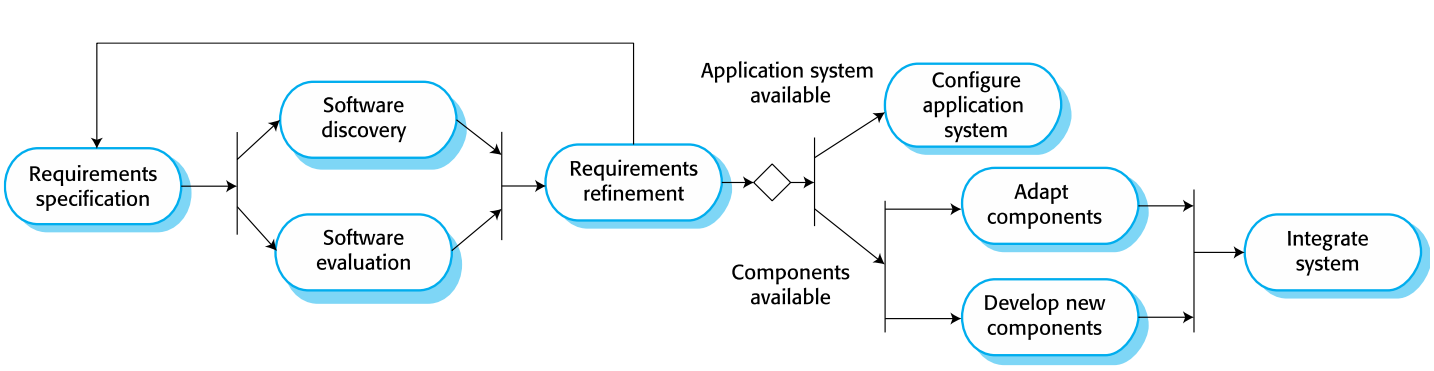
\includegraphics[width = 1.10\textwidth]{Images/13.png}
\end{center}
\newpage
\noindent
Vediamo ora i vantaggi e gli svantaggi di questo approccio:
\begin{itemize}
    \item \textbf{Vantaggio}: Riduzione dei costi e dei rischi, poiché \textbf{viene sviluppato meno software da zero}
    \item \textbf{Vantaggio}: Consegna più rapida del sistema al cliente
    \item \textbf{Svantaggio}: Si dovranno attuare dei \textbf{compromessi sui requisiti}, quindi il sistema potrebbe non soddisfare appieno le esigenze dell'utente
    \item \textbf{Svantaggio}: Perdita di controllo sull'\textbf{evoluzione} delle varie componenti che formano il sistema
\end{itemize}
\subsubsection{Processo a cascata}
\begin{center}
    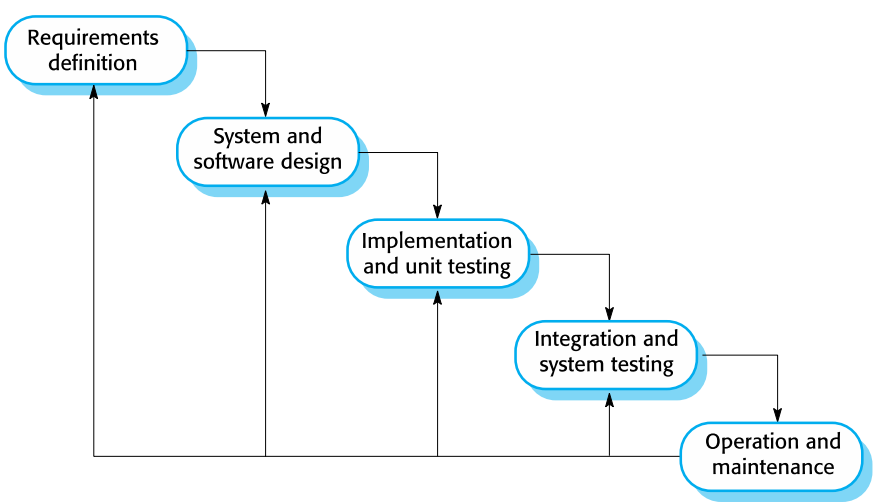
\includegraphics[width = 0.80\textwidth]{Images/14.png}
\end{center}
Il processo a cascata è il processo software \textbf{più vecchio} tra quelli utilizzati ancora oggi.
Il processo software con ciclo di vita a cascata (o \textbf{sequenziale}) è, in prima approssimazione, basato su uno svolgimento \textbf{sequenziale delle diverse attività di sviluppo del software}.
All'inizio di un progetto, vengono definiti in dettaglio \textbf{tutti i requisiti} (o almeno la maggior parte di essi); allo stesso modo, più o meno all'inizio del progetto, si cerca di stabilire un \textbf{piano temporale dettagliato e "affidabile"} delle attività da svolgere (non è detto che lo sia).
Poi si prosegue con la \textbf{modellazione} (analisi e progettazione) e viene creato un \textbf{progetto completo del software}. Solo a questo punto inizia la \textbf{programmazione del sistema software}, a cui seguiranno \textbf{verifica, rilascio e manutenzione}. Si noti come \textbf{ogni fase descritta inizia solo quando la precedente finisce}.
Ad essere precisi, il processo a cascata \textbf{permette la possibilità di feedback e cicli tra le attività}, ma la maggior parte delle organizzazioni che applica questo processo considera di solito una \textbf{sequenzialità stretta} fra le varie fasi.
Il principale svantaggio del processo a cascata è quindi quello di \textbf{avere difficoltà ad accogliere i cambiamenti a processo avviato}.
Il processo a cascata, tuttavia, \textbf{risulta una pratica mediocre per la maggior parte dei progetti software} ([Larman03] e [LB03]): infatti il processo a cascata è associato ad una \textbf{percentuale elevata di fallimenti}. Perché quindi questo processo è così soggetto a frequenti fallimenti?
\begin{itemize}
    \item La suddivisione \textbf{inflessibile} del progetti in \textbf{fasi distinte} rende difficile rispondere alle mutevoli esigenze di un cliente
    \begin{itemize}
        \item Pertanto, questo modello è appropriato \textbf{solo quando i requisiti sono ben compresi e le modifiche saranno piuttosto limitate durante il processi di sviluppo}. Questo però non accade, come mostrato dal seguente grafico dello studio [Jones97]:
        \begin{center}
            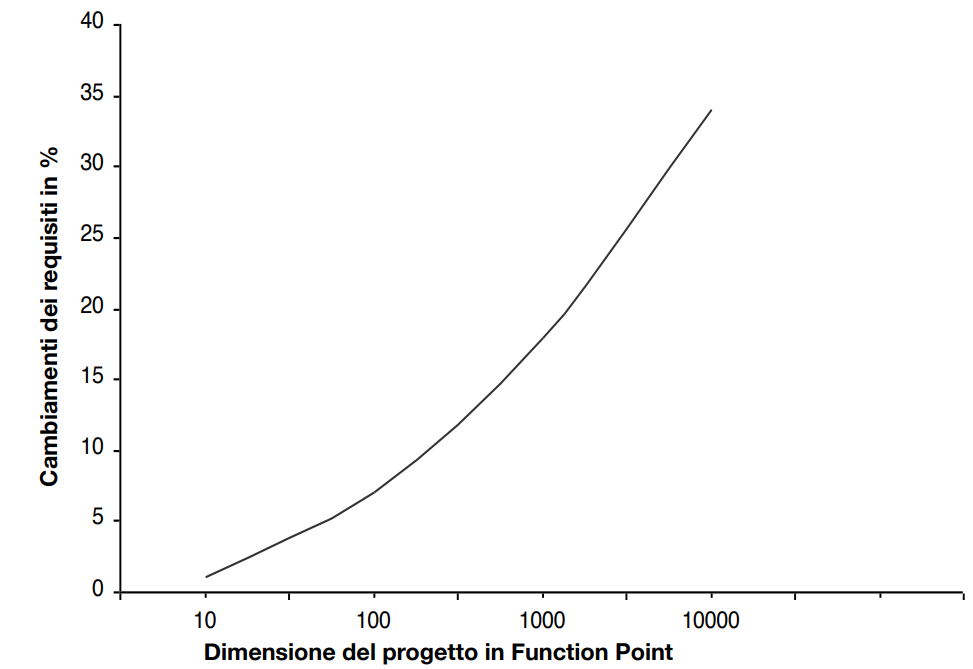
\includegraphics[width = 0.70\textwidth]{Images/15.png}
        \end{center}
    \end{itemize}
    \item Il modello a cascata viene utilizzato principalmente per progetti di \textbf{ingegneria dei sistemi di grandi dimensioni}, in cui un sistema viene sviluppato in diversi siti.
    \begin{itemize}
        \item In questo caso, la natura pianificata del processo a cascata \textbf{aiuta a coordinare il lavoro}
    \end{itemize}
\end{itemize}
\subsubsection{Sviluppo iterativo, incrementale ed evolutivo}
Una pratica fondamentale di molti processi software moderni (come UP e SCRUM) è lo \textbf{sviluppo iterativo}.
In questo approccio al ciclo di vita, lo sviluppo è suddiviso in \textbf{una serie di mini progetti} dalla durata temporale fissa (es. 3 settimane, si dicono quindi \textbf{timeboxed}) chiamate \textbf{iterazioni};
il risultato di ciascuna iterazione è \textbf{un sistema eseguibile, testato e integrato, ma parziale}. Ciascuna iterazione prevede le proprie fasi di \textbf{analisi dei requisiti, progettazione, implementazione e test}.
Il ciclo di vita iterativo si basa sul \textbf{susseguirsi di ampliamenti e raffinamenti} di un sistema nel corso di \textbf{molteplici iterazioni}, con \textbf{feedback e adattamenti ciclici} come guide essenziali per \textbf{convergere verso un sistema appropriato}.
Il sistema quindi \textbf{cresce in modo incrementale} nel tempo. Poiché il feedback e l'adattamento fanno \textbf{evolvere il sistema nel tempo}, questo processo si dice anche \textbf{evolutivo}.
\begin{center}
    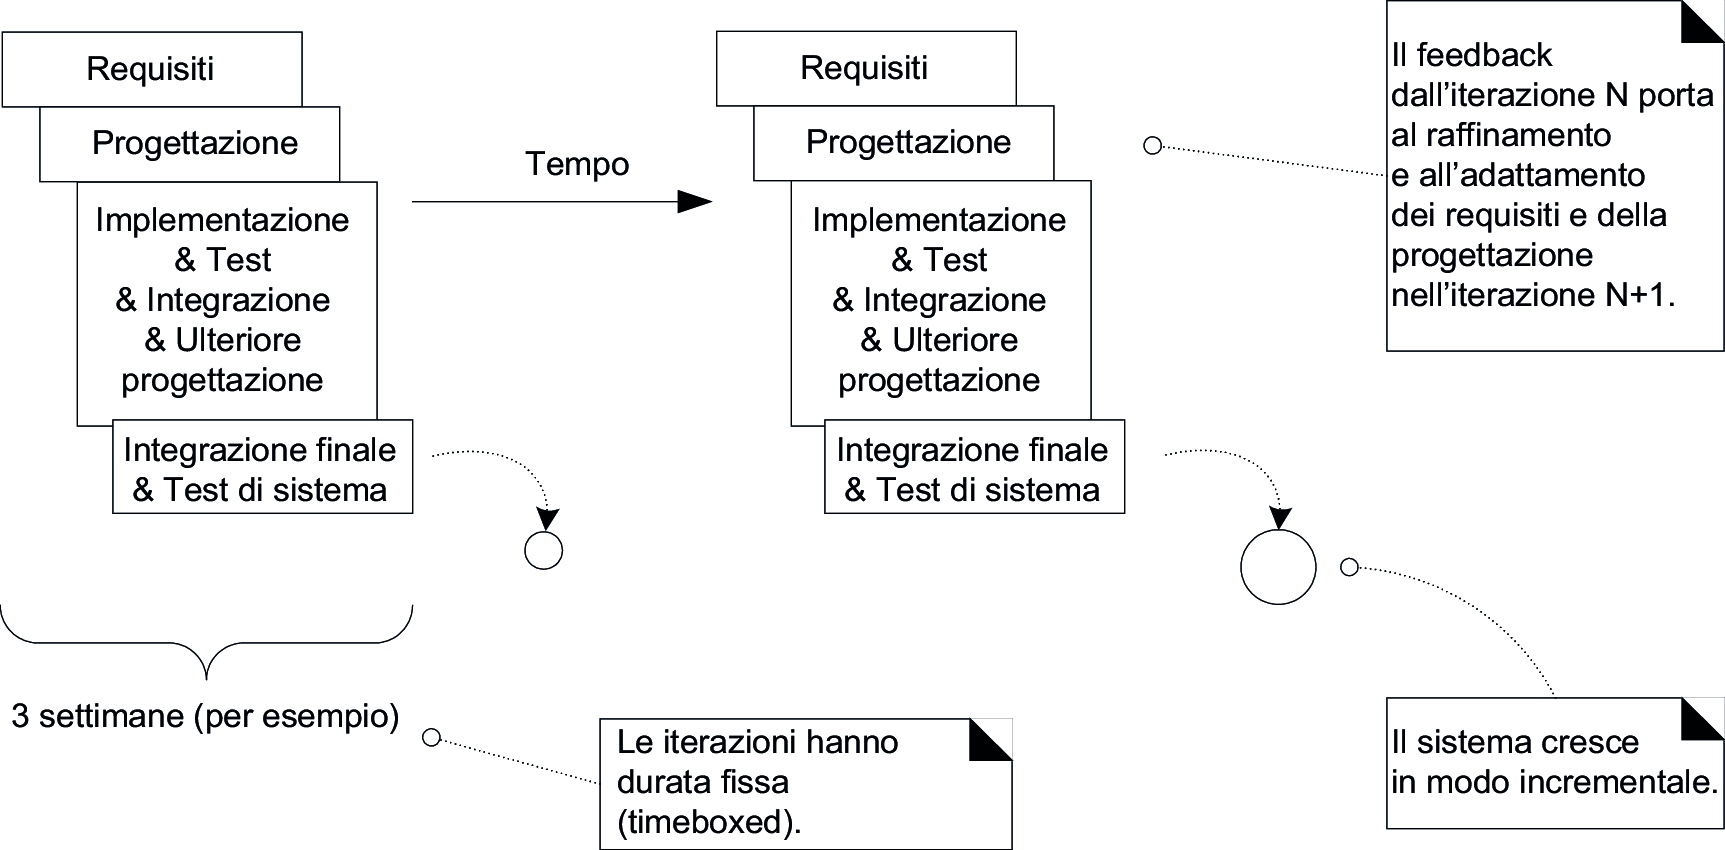
\includegraphics[width = 1\textwidth]{Images/16.png}
\end{center}
Quindi lo sviluppo iterativo, incrementale ed evolutivo si basa su un atteggiamento di \textbf{accettazione del cambiamento} e sull'\textbf{adattamento} come guide \textbf{inevitabili e di fatto essenziali}.
Tuttavia questo non significa che questo processo supporti uno sviluppo \textbf{caotico} e che gli sviluppatori continuino a cambiare direzione in base alle richieste estemporanee del cliente ("feature creep"). Una via di
mezzo \textbf{è possibile}:
\begin{itemize}
    \item Ciascuna iterazione comporta la scelta di un \textbf{di un piccolo sottoinsieme di requisiti, una rapida progettazione, implementazione e test}.
    Seppur nelle iterazioni iniziali ciò che si produce \textbf{sarà lontano da ciò che si vuole ottenere}, ciò permette al cliente di dare feedback in maniera \textbf{rapida e precoce}; i quali potranno essere \textbf{analizzati dal team di lavoro} per ottenere delle \textbf{indicazioni pratiche e significative}; ciò permette al team anche di avere un'opportunità di \textbf{modificare o adattare la comprensione dei requisiti e il progetto}.
    Oltre al chiarimento dei requisiti, attività quali i \textbf{test di carico} dimostreranno se il progetto e l'implementazione parziale sono nella direzione giusta o se è necessaria una modifica dell'architettura.
    \item Il lavoro procede mediante una serie di \textbf{cicli strutturati di costruzione-feedback-adattamento}
    \item Nel tempo, attraverso il \textbf{feedback iterativo} e \textbf{l'adattamento}, il sistema sviluppato \textbf{evolve} e \textbf{converge} verso i requisiti corretti e il progetto più appropriato
    \begin{itemize}
        \item Non bisogna stupirsi se nelle prime iterazioni lo \textbf{scostamento} dal sistema desiderato è maggiore che in quelle successive
        \item L'instabilità dei requisiti e del progetto \textbf{tende a diminuire nel tempo}, tuttavia nelle iterazioni finali è \textbf{difficile ma non impossibile} che si verifichi un \textbf{cambiamento significativo dei requisiti}
    \end{itemize}
\end{itemize}
Quali sono quindi i \textbf{vantaggi} dello sviluppo iterativo, incrementale ed evolutivo?
\begin{itemize}
    \item \textbf{Minore probabilità di fallimento del progetto}, \textbf{migliore produttività}, \textbf{percentuali più basse di difetti}
    \item Riduzione precoce, anziché tardiva, dei \textbf{rischi maggiori} (tecnici, requisiti obbiettivi ecc...)
    \item Progresso visibile \textbf{sin dall'inizio}
    \item \textbf{Feedback precoce}, coinvolgimento dell'utente e adattamento, che portano a un sistema che soddisfa al meglio le esigenze reali delle parti interessate
    \item \textbf{Gestione della complessità}, cioè il team non viene sopraffatto dalla "\textbf{paralisi da analisi}" o da \textbf{passi molto lunghi e complessi}
    \item Ciò che si apprende nel corso di un iterazione \textbf{può essere usato per migliorare le successive}
\end{itemize}
Tuttavia questo processo \textbf{non è privo di svantaggi}:
\begin{itemize}
    \item Il processo \textbf{non è visibile}: i manager hanno bisogno di documenti \textbf{costanti} per tenere traccia del processo di sviluppo; tuttavia se il sistema continua a cambiare non è conveniente continuare a produrre documenti che riflettono ogni versione del sistema
    \item La struttura del sistema \textbf{tende a degradarsi} con l'aggiunta di nuovi incrementi: a meno che non si dedichi tempo e denaro al \textbf{refactoring} per migliorare il software, le aggiunte tendono a \textbf{corrompere la struttura del sistema}; quindi incorporare sempre più modifiche software diventa sempre più \textbf{difficile e costoso}
\end{itemize}
Lo sviluppo iterativo è basato sul fatto che nei sistemi complessi e mutevoli, il feedback e l'adattamento sono \textbf{incrementi chiave} per il successo:
\begin{itemize}
    \item Feedback proveniente dalle \textbf{attività iniziali di sviluppo}, dai \textbf{programmatori} che cercano di leggere le specifiche e da \textbf{dimostrazioni ai clienti} per raffinare i requisiti
    \item Feedback proveniente dai \textbf{test} e dagli \textbf{sviluppatori} che raffinano il progetto e i modelli
    \item Feedback circa \textbf{l'avanzamento del team} nell'affrontare le prime caratteristiche, per raffinare le \textbf{stime di tempo e di costi}
    \item Feedback proveniente dal \textbf{cliente e dal mercato} per assegnare/modificare le \textbf{priorità} alle caratteristiche da affrontare nell'iterazione successiva
\end{itemize}
Una pratica fondamentale dello sviluppo iterativo è quella di avere \textbf{iterazioni di lunghezza fissata}, cioè \textbf{timeboxed}; il periodo consigliato è dalle \textbf{due alle sei settimane}.
Iterazioni più lunghe sono invece contrarie allo spirito dello sviluppo iterativo, poiché esso richiede \textbf{un feedback costante da parte del cliente}; con un periodo più lungo di sei settimane la complessità \textbf{cresce} e il feedback viene \textbf{ritardato}.
Iterazioni più corte di due settimane invece \textbf{difficilmente permettono di sviluppare abbastanza software} per avere un feedback significativo.
In questo processo di sviluppo \textbf{non è consentito ritardare la fine di un'iterazione}: se risulta difficile portare a termine tutti i requisiti che si erano previsti per una particolare iterazione, è meglio \textbf{spostarli all'iterazione successiva} piuttosto che modificare la durata dell'iterazione.
Un'iterazione di durata fissa è detta \textbf{timeboxed}. \newline
Bisogna anche fare attenzione che il \textbf{pensiero a cascata non si infiltri nello sviluppo iterativo}; segni di questa infiltrazione sono:
\begin{itemize}
    \item Si è scritto \textbf{la maggior parte dei requisiti o dei casi d'uso} prima dello sviluppo
    \item Si è creato in modo \textbf{dettagliato e completo delle specifiche, dei modelli o il progetto} prima di iniziare l'implementazione 
\end{itemize}
L'adozione dello sviluppo iterativo richiede che il software venga realizzato in modo \textbf{flessibile}, affinche l'impatto dei cambiamenti sia \textbf{il più basso possibile}. A tal fine il codice (e il progetto del software) devono essere \textbf{facilmente modificabili}.
Per facilitare questo aspetto il codice deve essere quindi \textbf{leggibile e facilmente comprensibile}, la mancanza di questa qualità infatti rende difficile implementare i cambiamenti in modo incrementale; inoltre è necessario usare degli \textbf{strumenti metodologici opportuni}; per esempio \textbf{tecnologie ad oggetti, sviluppo guidato dai test e refactoring}.
Vediamo un esempio visuale sul come avviene uno sviluppo iterativo, incrementale ed evolutivo se assumiamo 20 iterazioni (assumiamo di star seguendo UP):
\begin{center}
    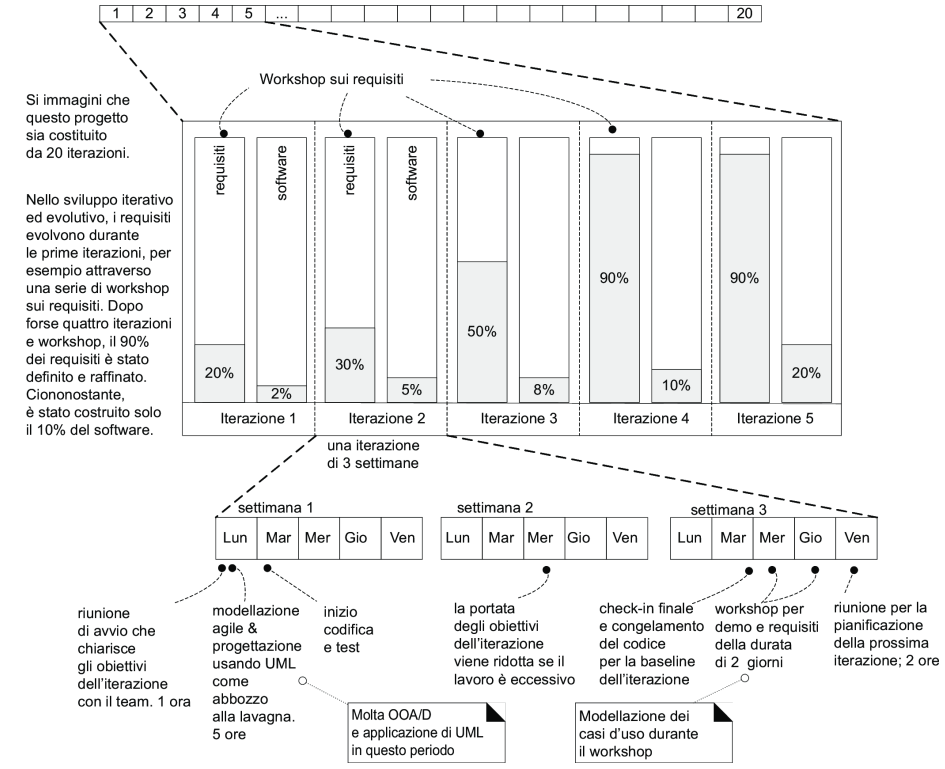
\includegraphics[width = 1.10\textwidth]{Images/17.png}
\end{center}
Un'attività critica dello sviluppo iterativo è la \textbf{pianificazione delle iterazioni}, cioè la definizione delle \textbf{attività da svolgere in ogni iterazione}.
Se si sta seguendo un processo iterativo, è necessario evitare di \textbf{tentare di pianificare l'intero progetto in modo dettagliato sin dalla prima iterazione}.
Piuttosto, i processi iterativi promuovono una \textbf{pianificazione iterativa} (o adattiva), in cui in ciascuna iterazione viene stabilito il \textbf{piano di lavoro dettagliato di una singola iterazione}.
In UP, la pianificazione viene effettuata alla \textbf{fine dell'iterazione corrente} per decidere le attività della \textbf{seguente iterazione}. In SCRUM, la pianificazione viene effettuata \textbf{all'inizio dell'iterazione} per stabilire il piano dell'iterazione \textbf{corrente}.
Lo sviluppo iterativo promuove la pianificazione \textbf{guidata dal rischio e guidata dall'utente}.
Ciò significa che gli obbiettivi delle iterazioni iniziali vengono scelti
\begin{enumerate}
    \item Per \textbf{identificare e attenuare i rischi maggiori}
    \item Per \textbf{costruire e rendere visibili} le caratteristiche a cui il cliente tiene di più
\end{enumerate}
In particolare, la progettazione guidata dal rischio contiene in sè la pratica dello \textbf{sviluppo centrato sull'architettura}: le prime iterazioni si concentreranno sulla \textbf{costruzione, test e la stabilizzazione del nucleo dell'architettura}.
Infatti, è un rischio molto alto \textbf{non avere un'architettura di base solida}. \newline
Importante per il processo iterativo è il \textbf{non cambiare gli obbiettivi dell'iterazione}: durante ciascuna iterazione, i requisiti su cui operare \textbf{vengono prima fissati} (pianificazione iterativa) e poi \textbf{bloccati}, cioè non sono più modificabili.
Durante ciascuna iterazione, quindi, il team \textbf{può lavorare al suo meglio}, poiché:
\begin{itemize}
    \item I requisiti sono \textbf{bloccati}, quindi il team non può essere \textbf{nè interrotto ne disturbato durante l'iterazione}
    \item I committenti possono interagire con il team di sviluppo \textbf{solo alla fine dell'iterazione}
\end{itemize}
Durante un'iterazione è tuttavia possibile che il team di sviluppo decida di \textbf{cambiare il piano dell'iterazione}, per esempio quando valuta, a metà dell'iterazione, la possibilità di raggiungere gli obbiettivi prefissati nella durata prevista.
\section{Unified Process (UP)}
Il \textbf{processo unificato} (unified process) o \textbf{UP} è un processo iterativo diffuso per lo sviluppo software orientato agli oggetti.
UP è molto \textbf{flessibile e aperto}: incoraggia infatti l'uso di \textbf{altre pratiche} prese da \textbf{altri processi iterativi}, come SCRUM o Extreme Programming.
UP è:
\begin{itemize}
    \item \textbf{Pilotato dai casi d'uso} (requisiti) e dai \textbf{fattori di rischio}
    \item Incentrato \textbf{sull'architettura}
    \item \textbf{Iterativo, incrementale ed evolutivo}
\end{itemize}
L'idea principale da apprezzare e praticare in UP è lo \textbf{sviluppo iterativo, evolutivo e incrementale} con \textbf{timeboxing breve}. Ulteriori best practices e concetti chiavi di UP sono:
\begin{itemize}
    \item Affrontare le problematiche di \textbf{rischio maggiore} e valore elevato nelle \textbf{iterazioni iniziali}
    \item Impegnare gli utenti \textbf{continuamente} sulla valutazione, il feedback e i requisiti
    \item Creare un'architettura \textbf{coesa} nelle iterazioni iniziali
    \item Verificare continuamente le \textbf{qualità}: testare \textbf{spesso, presto e in modo realistico}
    \item Applicare i \textbf{casi d'uso}, se appropriato
    \item Fare della \textbf{modellazione visuale} (con UML)
    \item Gestire attentamente i requisiti
    \item Gestire le richieste di cambiamento e le configurazione
\end{itemize}
Vediamo una sua breve storia:
\begin{center}
    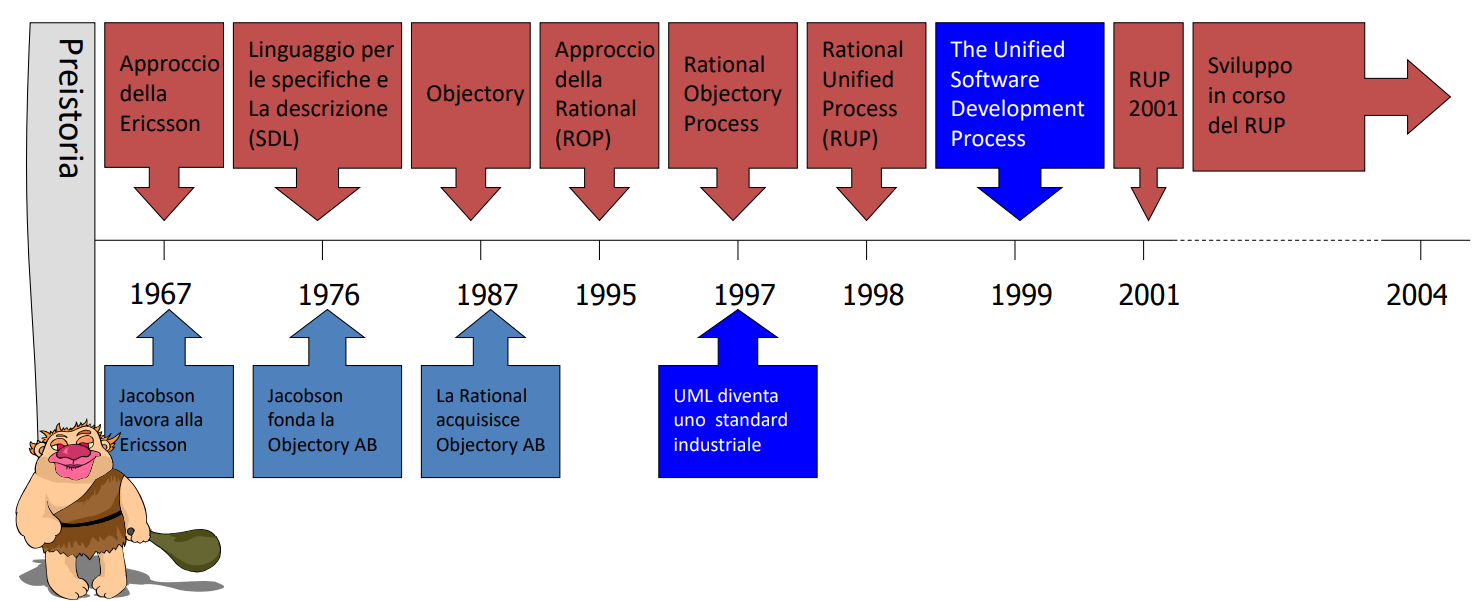
\includegraphics[width = 1\textwidth]{Images/18.png}
\end{center}
\subsection{Iterazioni e discipline}
Le iterazioni sono \textbf{concetti chiave} in UP. Esse sono come un mini-progetto che include:
\begin{itemize}
    \item \textbf{Pianificazione}
    \item \textbf{Analisi e progettazione}
    \item \textbf{Costruzione}
    \item \textbf{Integrazione e test}
    \item \textbf{Un rilascio}
\end{itemize}
Poiché UP è un processo iterativo, si arriva al \textbf{rilascio finale} dopo una \textbf{serie di iterazioni}. 
Le iterazioni \textbf{possono sovrapporsi}; ciò permette lo \textbf{sviluppo parallelo e il lavoro flessibile in grandi squadre}.
Tuttavia richiede un'attenta pianificazione. \newline
UP colloca le attività lavorative in \textbf{discipline}; una disciplina è \textbf{un insieme di attività e dei relativi elaborati in una determinata area}, come, per esempio, l'area dell'analisi dei requisiti.
In UP, un \textbf{elaborato} è il termine generico con cui si fa riferimento ad un qualsiasi \textbf{prodotto di lavoro} (codice, schema di basi di dati, ecc...).
UP definisce diverse discipline ed elaborati, ma noi ci concentreremo su:
\begin{itemize}
    \item \textbf{Modellazione di business}: L'elaborato \textbf{Modello di dominio}, per visualizzare i concetti significativi nel dominio di applicazione
    \item \textbf{Requisiti}: Gli elaborati \textbf{Modello dei casi d'uso e Specifica supplementare}, per descrivere i \textbf{requisiti funzionali e non funzionali}
    \item \textbf{Progettazione}: L'elaborato \textbf{Modello di progetto}, per il progetto degli oggetti software
\end{itemize}
Un elenco più ampio è il seguente:
\begin{center}
    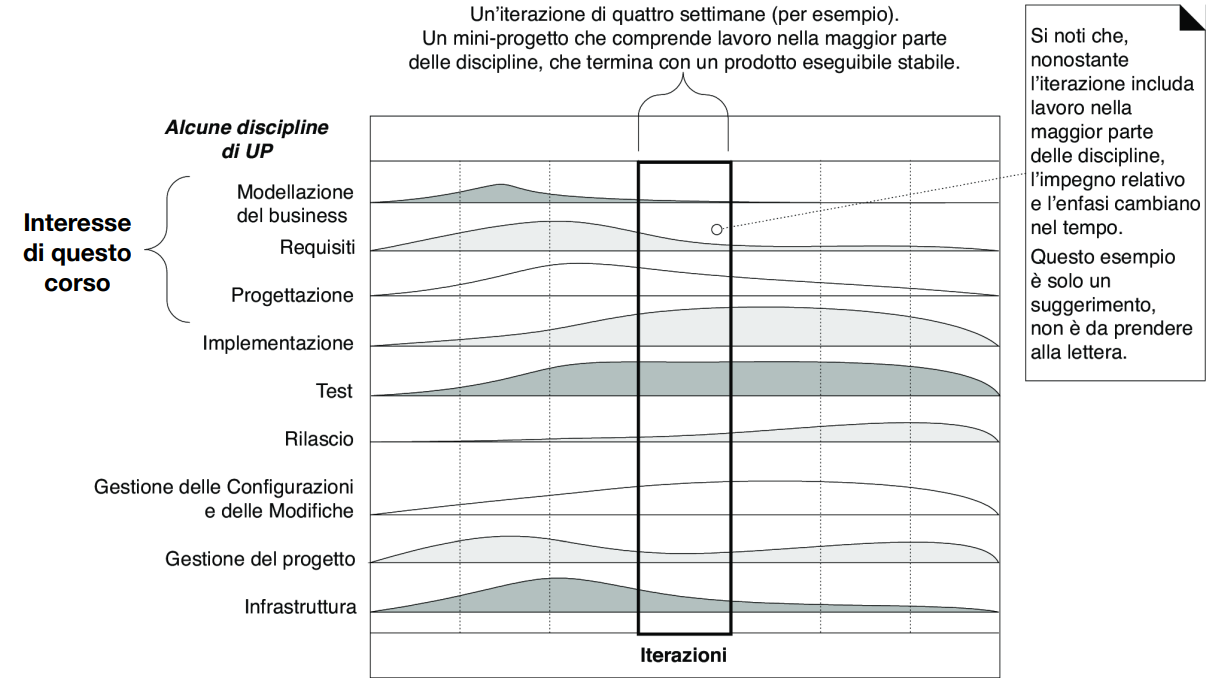
\includegraphics[width = 1.10\textwidth]{Images/19.png}
\end{center}
Come si può vedere sopra, anche se ogni iterazione può prevedere \textbf{tutti i flussi di lavoro}, la collocazione dell'iterazione all'interno del ciclo di vita del progetto \textbf{determina una maggiore enfasi} su uno dei flussi di lavoro.
\subsubsection{Release}
Ogni iterazione \textbf{genera una release}: una release è un \textbf{insieme di manufatti}, previsti e approvati. Essa fornisce una \textbf{base approvata per le successive attività di analisi e sviluppo}.
Un \textbf{incremento} è la \textbf{differenza} tra una release e la successiva. Costituisce quindi un passo in avanti verso il rilascio finale del sistema.
\newpage
\subsection{Fasi di UP}


\end{document}
